\documentclass[11pt,a4paper]{article}
\usepackage[useregional]{datetime2}
\usepackage{needspace}


% Date Time
\DTMsetdatestyle{iso}

% Utilisation du style SOBA (défini dans soba.sty)
\input{@@STYLE_FILE@@.sty}
\graphicspath{{@@GRAPHICS_DIRECTORY@@/}}
% soba.sty loads hyperref without options, which draws a red box around every
% cross-reference, table-of-contents entry and URL.
\hypersetup{hidelinks}
\geometry{top=2.6cm,headheight=44pt,headsep=15pt}
% This document describes a curated dataset, so it overrides the style's
% default co-aligned catalogue footer.
\lfoot{Curated Dataset Description - Ifremer}

% ---------------------------
% DÉBUT DU DOCUMENT
% ---------------------------
\begin{document}

% Page de garde
\begin{titlepage}
    \centering
    \vspace*{2cm}

    % Logo
    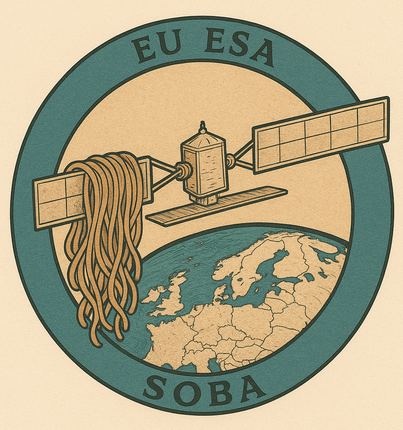
\includegraphics[width=0.4\textwidth]{logo_soba.png}

    \vspace{2cm}

    {\Huge \textbf{SOBA Project} \par}
    \vspace{1cm}
    {\Large \textbf{Technical documentation for @@DATASET_NAME@@ curated dataset} \par}

    \vspace{2cm}

    \textbf{Work Package 3: Datasets Preparation} \\
    \vspace{0.5cm}

    \begin{minipage}{0.85\textwidth}
        \textbf{Scope:} @@SCOPE_TEXT@@
    \end{minipage}

    \vfill

    \begin{center}
    \begin{tabular}{ll}
        \textbf{Document Version} & 1.1.0 \\
        \textbf{Date} & \DTMtoday \\
        \textbf{Authors} & SOBA consortium \\
        \textbf{Intended Audience} & internal \\
    \end{tabular}
    \end{center}

    \vspace{1cm}
\end{titlepage}

\tableofcontents

\newpage

% The supplied PNG contains its own Figure 1 caption; count it without a duplicate.
\begin{figure}[H]
    \centering
    \refstepcounter{figure}\label{fig:dataflow}
    \includegraphics[width=\textwidth,height=0.72\textheight,keepaspectratio]{@@DATAFLOW_FIGURE@@}
\end{figure}

\section*{Version History}
\addcontentsline{toc}{section}{Version History}

\begin{table}[H]
    \centering
    \caption{Versioning of the documentation}
    \label{tab:versioning_documentation}
    \begin{tabular}{@{}p{1.3cm}p{2cm}p{6.9cm}p{2.5cm}p{2.1cm}@{}}
        \toprule
        \textbf{Version} & \textbf{Date} & \textbf{Modification} & \textbf{Author} & \textbf{Checked by} \\
        \midrule
        1.0.0 & \DTMtoday & Creation of the @@DOCUMENT_PRODUCT@@ curated dataset document & Ilias Reguig & -- \\
        1.1.0 & \DTMtoday & Public-facing sources and selection summary & Ilias Reguig & -- \\
        \bottomrule
    \end{tabular}
\end{table}

\begin{table}[H]
    \centering
    \caption{Versioning of curated catalogue files}
    \label{tab:versioning_catalogue_files}
    {\small
    \begin{tabular}{@{}>{\raggedright\arraybackslash}p{7cm}p{2cm}>{\raggedright\arraybackslash}p{7cm}@{}}
        \toprule
        \textbf{File name} & \textbf{Date} & \textbf{Modifications} \\
        \midrule
        @@FILE_VERSION_ROW@@
        \bottomrule
    \end{tabular}
    }
\end{table}


% ---------------------------
% SECTION 1 : Dataset Content Description
% ---------------------------

\section{Dataset Content Description}
\textbf{Dataset general description:} @@GENERAL_DESCRIPTION@@

\subsection{Global Coverage Map}
\textbf{Description:} @@COVERAGE_DESCRIPTION@@
\begin{figure}[H]
    \centering
    \includegraphics[width=\textwidth]{@@COVERAGE_FIGURE@@}
    \caption{@@COVERAGE_CAPTION@@}
    \label{fig:coverage_map}
\end{figure}

\Needspace{0.43\textheight}
\subsection{Monthly Distribution of Matchups}
\textbf{Description:} @@MONTHLY_DESCRIPTION@@
\begin{figure}[H]
    \centering
    \includegraphics[width=0.85\textwidth]{@@MONTHLY_FIGURE@@}
    \caption{@@MONTHLY_CAPTION@@}
    \label{fig:monthly_distribution}
\end{figure}

\Needspace{0.43\textheight}
\subsection{@@DISTRIBUTION_TITLE@@}
\textbf{Description:} @@REFERENCE_DESCRIPTION@@
@@DISTRIBUTION_FIGURES@@

Table~\ref{tab:reference_stats} summarises the retained @@REFERENCE_LABEL@@.
@@REFERENCE_STATS_TABLE@@

\Needspace{0.98\textheight}
\subsection{Catalogue Columns}
Table~\ref{tab:columns} gives the columns and stored types of the Curated Parquet files, including source reference measurements and curation provenance. Descriptions marked inferred are field-name interpretations, not verified source definitions.
\begin{table}[H]\centering
\caption{Columns of the Curated Parquet files.}
\label{tab:columns}
{\footnotesize
\begin{tabular}{@{}>{\raggedright\arraybackslash}p{4.1cm}>{\raggedright\arraybackslash}p{2.6cm}>{\raggedright\arraybackslash}p{8.1cm}@{}}
\toprule
\textbf{Column} & \textbf{Type} & \textbf{Description} \\
\midrule
@@TEST_COLUMNS@@
\bottomrule
\end{tabular}
}
\end{table}

@@SAMPLING_NOTE@@

\Needspace{0.65\textheight}
\subsection{Global Metadata}
Product metadata and provenance are listed below. Original source attributes remain in the Parquet files; run-specific provenance is recorded in the accompanying manifest.
\begin{table}[H]\centering
\caption{Global attributes of the parquet files.}
\label{tab:metadata}
{\small
\begin{tabular}{@{}>{\raggedright\arraybackslash}p{5.4cm}>{\raggedright\arraybackslash}p{8.9cm}@{}}
\toprule
\textbf{Attribute} & \textbf{Value} \\
\midrule
@@METADATA_ROWS@@
\bottomrule
\end{tabular}
}
\end{table}

% ---------------------------
% SECTION 2 : Dataset Production Steps
% ---------------------------
\section{Dataset Production Steps}
\subsection{Selected Products}
\begin{itemize}
    \item \textbf{SAR product and provider:} @@SAR_PRODUCT@@
    \item \textbf{Reference product and provider:} @@REFERENCE_PRODUCT@@
    \item \textbf{SAR acquisition mode:} Wave Mode (WV).
    \item \textbf{Polarization:} single VV (SV).
\end{itemize}

\subsection{Selection of Tiles / Filtered Co-locations}
@@SELECTION_SUMMARY@@

\textbf{Date selection.} The date windows define the evaluation period included in this release, not the launch dates or full lifetimes of the satellites.
\begin{itemize}
@@DATE_SELECTION@@
\end{itemize}

@@SEQUENTIAL_COUNTS@@

@@DIRECTION_STD_NOTE@@

\begin{table}[H]
    \centering
    \caption{Matches before and after the additional selection.}
    \label{tab:selection_summary}
    \begin{tabular}{lrrr}
        \toprule
        \textbf{Mission} & \textbf{Before selection} & \textbf{Retained} & \textbf{Removed} \\
        \midrule
@@BEFORE_AFTER_ROWS@@
        \midrule
        Total & @@INPUT_COUNT@@ & @@ROW_COUNT@@ & @@REMOVED_COUNT@@ \\
        \bottomrule
    \end{tabular}
\end{table}
\textbf{Before selection} counts the space/time-matched observations available at the end of the first preparation stage; \textbf{retained} counts those left after the date selection and additional quality filters. Multiple reference matches can correspond to one SAR image, so row counts are not counts of distinct images.


\addcontentsline{toc}{section}{References}

\begin{thebibliography}{9}
@@PRODUCT_REFERENCES@@
\end{thebibliography}
\end{document}
